\documentclass[class=report, crop=false]{standalone}
\usepackage[subpreambles=true]{standalone}
\usepackage{import}

\begin{document}
\newpage
We have a GitHub organisation, where we have already published a lot of our current code. It can be found \href{https://github.com/CanOpeners}{here}. \\
\subsection*{Onboard Software}
We are going to use the C programming language for the onboard software. \\
We have already managed to retrieve information from all the sensors we have, including but not limited to the temperature sensor, the pressure sensor and the accelerometer. \\
We also have programmed the GPS and camera data retrieving software. \\
We are going to save all the data to an onboard SD card, and transmit as much data over the radio bandwidth as the connection will be able to handle. \\
We have yet to decide what exact format of protocol we will use for communication. \\
We are also going to have two way communication, so as to be able to control the satellite's submodules midflight.
\subsection*{Ground Station Software}
The ground station will of a main computer connected to a small microcontroller which will read and transfer radio communication to the main computer. \\
The microcontroller will also use the C programming language for it's software. \\
We will most likely use Python or Julia for the main computer's software. Were we to use create a GUI, we would use either GTK or just use the CLI libraries such as ncurses. \\

\subsection*{SatTrack Software}
The software of the SatTrack system will work in the following manner: \\
The ground antenna shall receive a signal from the satellite. The signal is going to contain various data, such as the on-board pressure readings and the GPS coordinates of the CanSat. \\
These two values are going to be used by the system to determine the angle of elevation and the direction of the ground antenna. \\
Afterwards, the program will subtract the ground station GPS coordinates from the coordinates it just received.
This way, the ground station will know the distance in each axis from the satellite. \\
With that knowledge, the ground station projects a right triangle, with its `legs' being the distanced in the $X$ and $Z$ axes. \\
Using basic trigonometry, the direction angle $\alpha$ is calculated by using a relation of $\tan\left(\alpha\right) = \frac{X}{Z}$. \\
The angle can be easily calculated using the $\arctan$ function. The elevation angle of the satellite is calculated analogically. \\
The $X$ and $Z$ coordinates are taken from the GPS, and the $Y$ distance is calculated from the on-board pressure readings. \\
The relation between the angle of elevation $\beta$ and the $X,Y,Z$ distances are as follows: $\tan\left(\beta\right) =\frac{Y}{\sqrt{X^2+Z^2}}$. This can also be calculated via the $\arctan$ function. \\

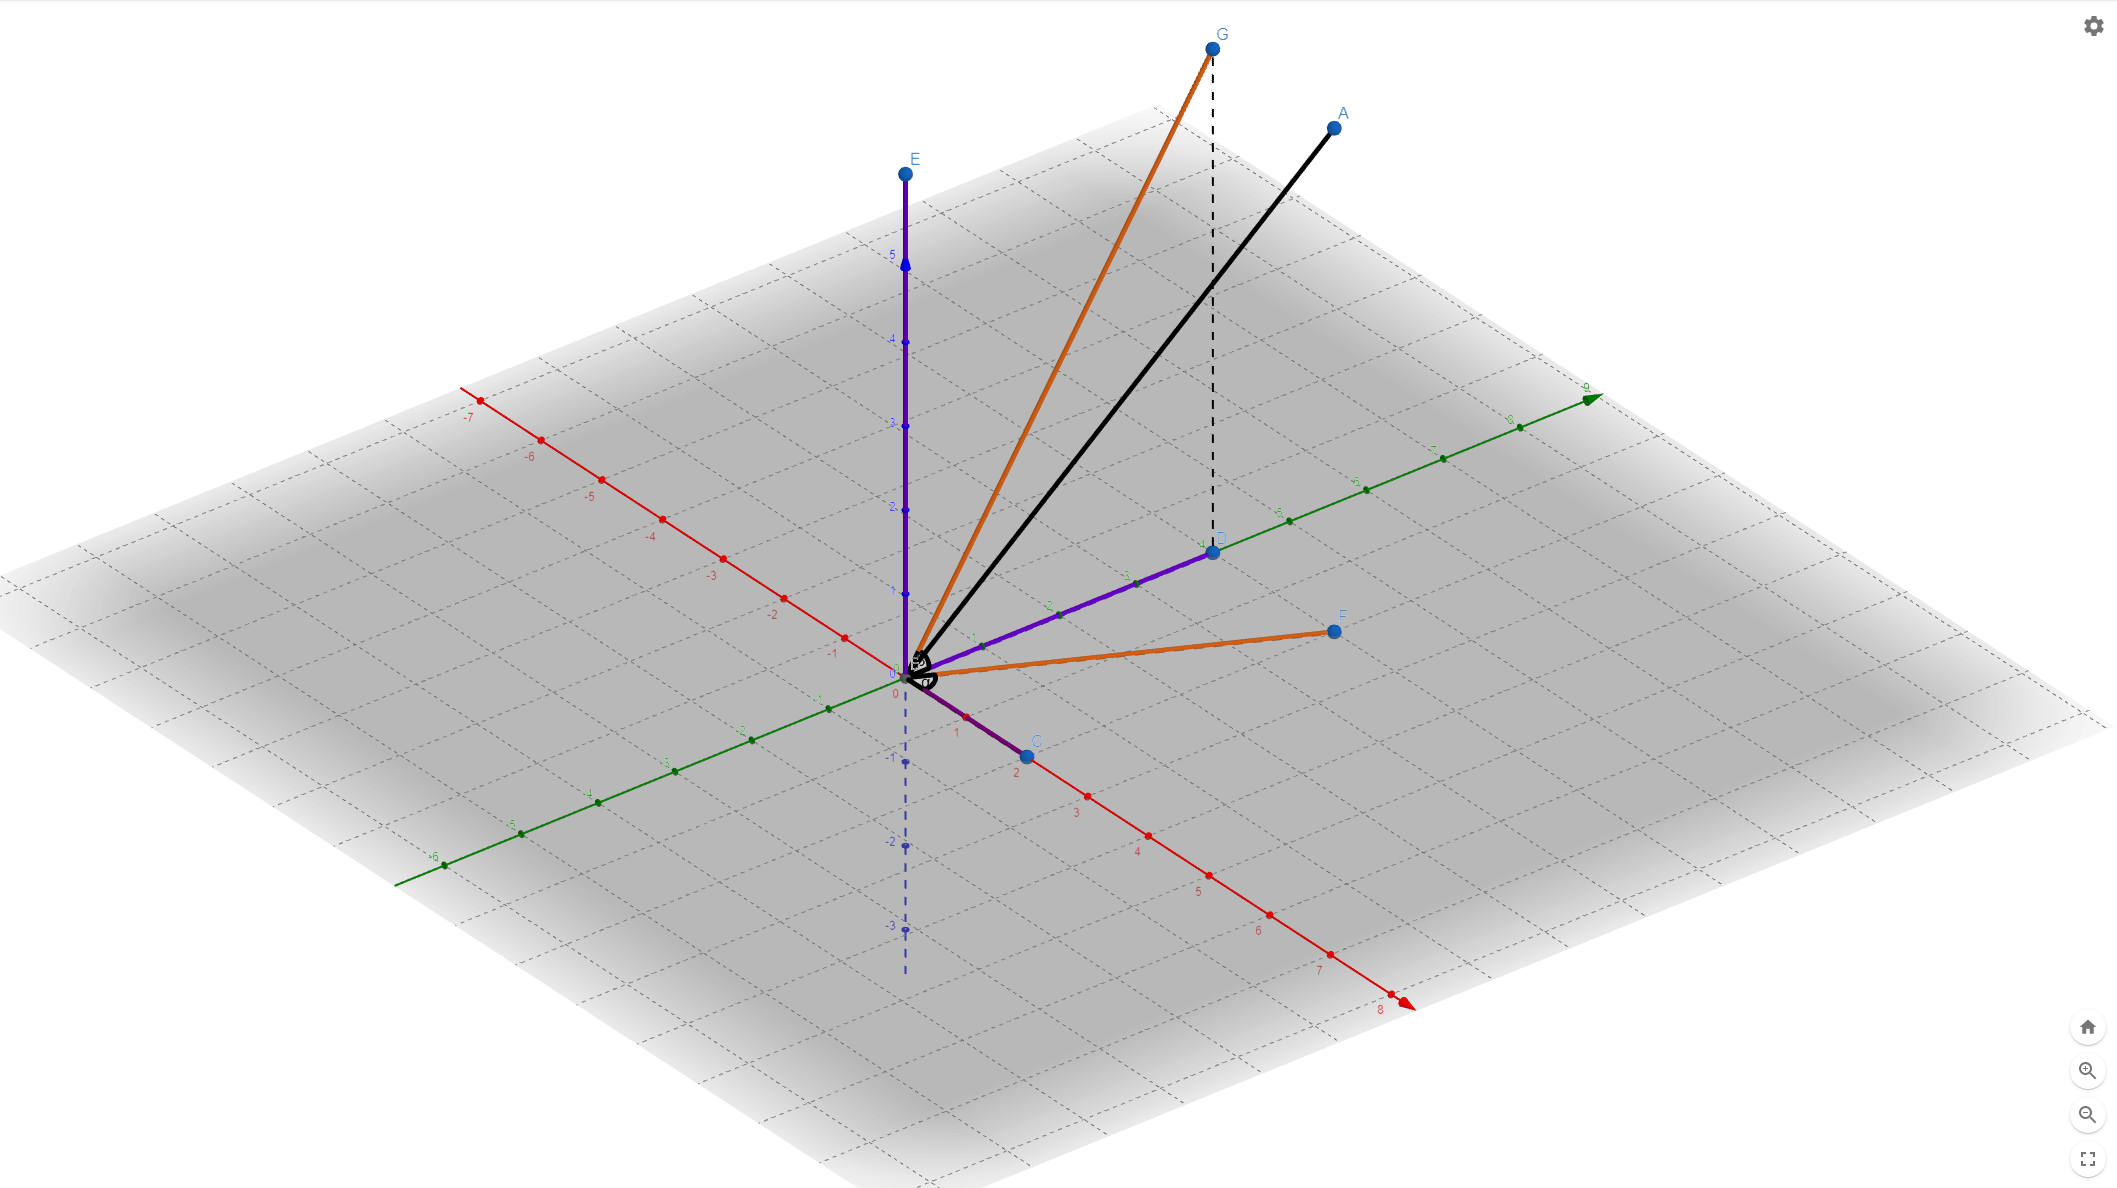
\includegraphics[width=\columnwidth]{ext/sattrackschema.png}
\captionof{figure}{A possible visualization of the vector triangulation process}
\end{document}
